\documentclass[10pt,a4paper,danish]{article}
\usepackage{amssymb}
\usepackage{amsmath}

\usepackage{palatino}

\usepackage[danish]{babel}
\usepackage[utf8]{inputenc}

\usepackage{alltt}

\usepackage{fancyref}

\usepackage{graphicx}
\usepackage{microtype}


\renewcommand{\Frefsecname}{Afsnit}
\renewcommand{\frefsecname}{afsnit}

\newcommand{\Frefexmname}{Eksempel}
\newcommand{\frefexmname}{eksempel}

\newcommand{\fancyrefexmlabelprefix}{exm}

%\fancyrefchangeprefix{\fancyrefeqlabelprefix}{exm}
\frefformat{vario}{\fancyrefexmlabelprefix}{
  \frefexmname\fancyrefdefaultspacing#1
}
\Frefformat{vario}{\fancyrefexmlabelprefix}{
  \Frefexmname\fancyrefdefaultspacing#1
}

\newcommand{\ct}{\texttt}


% Eksempel environment
\newtheorem{example}{Eksempel}[subsection]


\title{Graf Teori\\\small{version \input{version}}}
\author{Johan Brinch, zerrez@diku.dk}

\begin{document}

\maketitle
\newpage


\tableofcontents
\newpage

\section{Introduktion til grafer}
Grafen er en datastruktur. Af andre datastrukturer findes blandt andet
\ct{lister}, \ct{tupler} og \ct{dictionaries}.

Lister og tupler lagrer elementer i en rækkefølge,
f.eks. [1,0,2,1]. Dictionaries lagrer par af nøgler og værdier, så en
værdi kan findes ved opslag på dens tilhørende nøgle, f.eks. \{a: 1,
b: 0, c: 2, d: 1\}.

Grafer bruges til at beskrive forhold. Grafen indeholder elementer,
kaldet knuder, og forhold mellem par af elementer, kaldet kanter.  For
eksempel kunne en graf lagre personer hvis forhold er givet ved
hvorvidt to personer er venner eller ej. Hver knude ville symbolisere
en person og hver kant et venskab.


\begin{figure}[h]
\centering
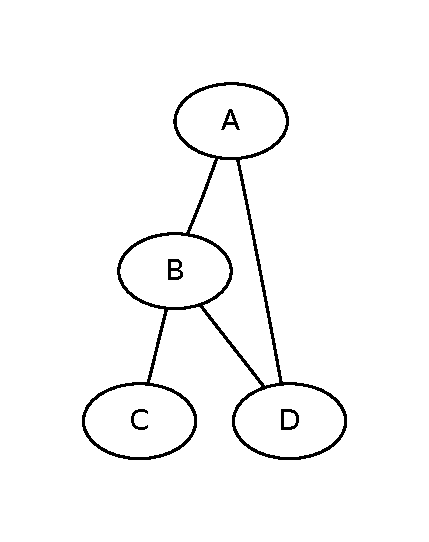
\includegraphics[width=.3\textwidth]{graphs/graph0.pdf}
\caption{Eksempel på graf}
\label{fig:graph0}
\end{figure}


\subsection{Knuder og kanter}
En graf består af knuder og kanter. Alle kanter forbinder to
knuder. En knude kan have nul eller flere kanter. Knuderne i grafen er
"`emnerne"', som grafen beskriver. Kanterne er deres relationer til
hinanden.


\begin{example}Metronettet\end{example}
  Et eksempel på en graf kunne være metronettet. Her kunne stationer
  repræsenteres som knuder og forbindelser imellem dem som kanter.

\begin{figure}[h]
\centering
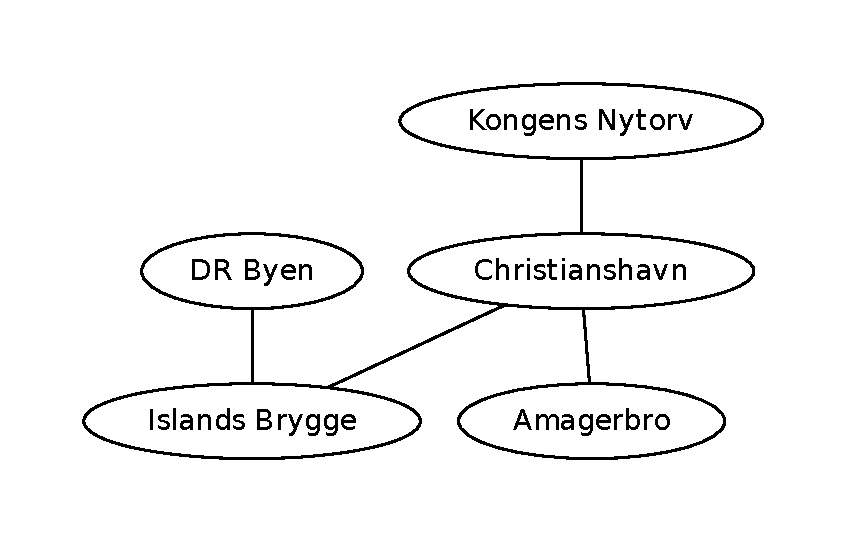
\includegraphics[width=.75\textwidth]{graphs/metro0.pdf}
\caption{Graf over et udsnit af metronettet}
\label{fig:metro0}
\end{figure}

\Fref{fig:metro0} viser en graf over metronettet med 5 knuder og 4
kanter. Knuderne er stationer og kanterne forbindelser. Grafen bruges
her til at vise hvilke stationer der er forbundet til hinanden.

Grafen kaldes retningsløs eller \textit{undirected} fordi kanterne
ikke angiver en retning. En forbindelse virker begge veje. Hvis man
kan tage toget fra Nørreport til Kongens Nytorv er det også muligt at
gå den anden vej. I en graf hvor kanterne angiver en retning (en
\textit{directed} graf) er det kun muligt at "`følge"' kanten i den
angivne retning. Forbindelsen virker kun den ene vej. Dens er
\textit{ensrettet}.

\subsection{Orienterede grafer}
En orienteret (\textit{directed}) graf er en graf hvori alle kanter
har en tilknyttet retning. Kanten kan nu kun følges i den angivne
retning. Det er dog muligt at tillade "`bevægelse"' mellem to knuder i
begge retninger, ved at tilføje to kanter: en i hver retning.

\begin{example}Metronettet udbygges med ensretning\end{example} Sæt
nu, at man vælger at bygge en ensrettet forbindelse mellem DR Byen og
Kongens Nytorv. Det er nu muligt at tage toget fra DR Byen til Kongens
Nytorv, men ikke den modsatte vej. Grafen over metronettet må dermed
laves med en orienteret graf, hvor alle kanter angiver en gyldig
retning. Ved de forbindelser, der tillader bevægelse i begge retninger
bruger vi to kanter. \Fref{fig:metro1} viser grafen fra
\fref{fig:metro0} udvidet med orientering og den nye kant.
\begin{figure}[h]
\centering
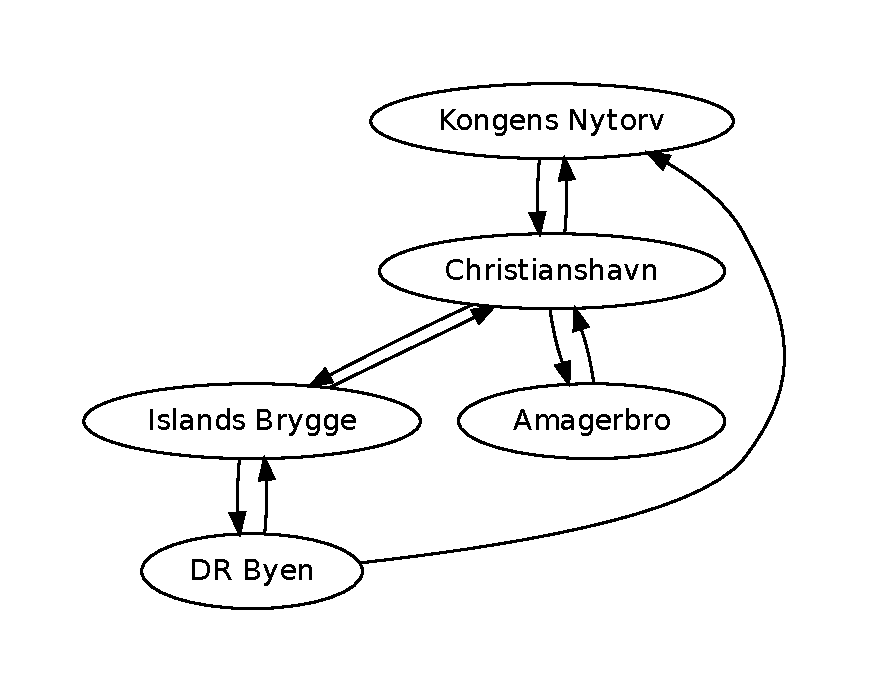
\includegraphics[width=.75\textwidth]{graphs/metro1.pdf}
\caption{Orienteret graf over metronet}
\label{fig:metro1}
\end{figure}

\subsection{Veje}
En vej i en graf er et sæt af knuder, der er forbundne af kanter.

\begin{example}
\label{exm:path}
Til DR Byen og tilbage igen\end{example}

\Fref{fig:metro0} viser en uorienteret graf over metronettet.
Betragt vejen:\\\indent
DR Byen $\to$ Islands Brygge $\to$ Christianshavn $\to$ Kongens Nytorv
\\

Det er den korteste vej (3 brugte kanter) mellem DR Byen og Kongens
Nytorv. Men det er ikke den eneste vej mellem de to stationer. Man
kunne havde taget forbi Amagerbro på vejen, blot for at vende om og
fortsætte mod Kongens Nytorv. Denne vej ville have brugt 5 kanter i
stedet for 3.

Hvis vi i stedet vender blikket mod den orienterede graf fra
\fref{fig:metro1}, ser vi at ovenstående ikke længere er den korteste
vej fra DR Byen til Kongens Nytorv. Vi kan nu gøre brug af den nye
direkte forbindelse og få vejen:\\\indent
DR Byen $\to$ Kongens Nytorv
\\

Vejen indeholder nu kun 1 kant (2 mindre). Desværre kan den direkte
forbindelse kun bruges i en retning, så tilbagevejen bliver noget
længere:\\\indent
Kongens Nytorv $\to$ Christianshavn $\to$ Islands Brygge $\to$
DR Byen\\

Tilbagevejen bruger igen 3 kanter.

\begin{example}Cykler\end{example} En vej kaldes en cykel
(\textit{cycle}) hvis start- og slutknuden er den samme. Vi kan
sammensætte de to veje fra \fref{exm:path} og få cyklen:\\\indent

DR Byen $\to$ Kongens Nytorv $\to$ Christianshavn $\to$ Islands Brygge
\\\indent $\to$ DR Byen\\

En vej kaldes en cykel, hvis den starter og slutter med samme
knude.


\subsection{Vægtede kanter}
Indtil nu har vi kun beskæftiget os med uvægtede grafer. I korteste
vej eksemplet fra \fref{exm:path} var længden af vejen antallet af
kanter der indgik i vejen. Man tænke på det, som at hver kant
kostede 1 at bruge.

I en vægtet graf tildeles hver kant en vægt (\textit{weight}), der
angiver hvor meget kanten koster. Man kan tænke på det som en
afstand mellem de to knuder kanten forbinder. Vægten angiver dermed
kantens længde.

Lad vende tilbage til metronettet. \Fref{fig:metro2} viser
\fref{fig:metro1} med angivede vægte. Hver vægt viser antallet af
minutter det tager at bevæge sig over den tilhørende kant.

Ifølge grafen tager den direkte vej fra DR Byen til Kogens Nytorv
5 minutter, mens den "`gamle"' vej, over Christianshavn, tager 6
minutter. Cyklen fra DR Byen til Kongens Nytorv og tilbage igen ville
altså tage 11 minutter at gennemføre.

\begin{figure}[h]\centering
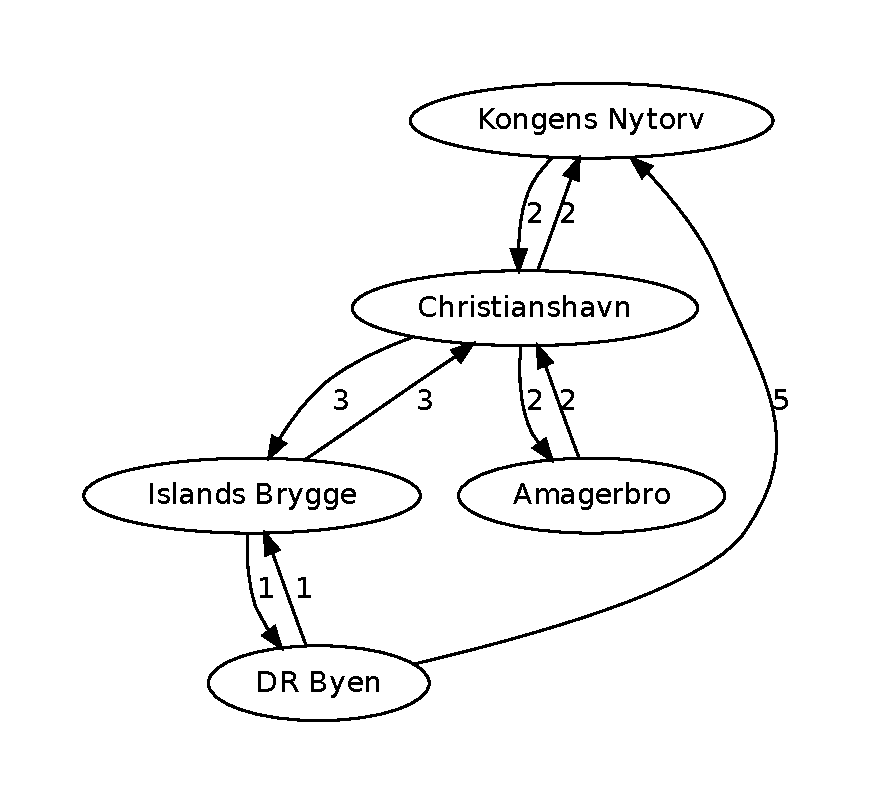
\includegraphics[width=.75\textwidth]{graphs/metro2.pdf}
\caption{Vægtet graf over metronet}
\label{fig:metro2}
\end{figure}




\subsection{Søgning i grafer}
Ligesom der kan søges i lister er det også muligt at søge i grafer. I
kan en søgning efter et element $a$ gøres ved at gennemløbe listen og
sammenligne alle elementer med $a$. Gennemløbet starter ved første
element og fortsætter herefter med næste element indtil listen løber
tør for elementer.

I Python kan liste-gennemløb udføres med en \ct{for}-løkke. Da listens
elementer er nummereret som første, andet, tredje $\dots$ $n$'e
element er rækkefølgen af elementerne oplagt.

I grafen er der ikke på samme måde en oplagt rækkefølge at udvælge
knuderne på. Der er ikke nogen $i$'e knude.

I de følgende afsnit skal vi se på to forskellige tilgange til søgning
i grafer, der hver definerer en rækkefølge, hvori knuderne kan
gennemløbes. Når først en sådan rækkefølge er klar kan søgning efter
knuden $a$ udføres ved sammenligning med hver knude (som ved
lister).

I \fref{sec:shortest_path} skal vi se hvordan gennemløb af grafer kan
bruges til at finde den korteste vej mellem to hustande i et vejnet.


\subsubsection{Dybde-først søgning}

I en dybde-først søgning (\textit{depth-first search}) defineres
rækkefølgen af knuder ved at vælge de "`dybe"' niveauer først (de knuder,
der ligger langt fra start-knuden).

I dybde-først søgning vælges en vilkårlig knude som start-knude, der
besøges først. Herefter vælges en vilkårlig kant (retning), der følges
så langt som muligt (rekursion). Når den valgte kant er fuldt
udforsket fortsætter søgningen med næste kant.

Der tages løbende højde for, at hver knude kun besøges \'en gang.

Dybde-først søgning kan også forstås på følgende måde:
\begin{enumerate}
\item Du står ved et vejkryds i en by og skal finde et specifik
  kryds. Du har ikke noget kort.
\item På skift prøver du hver vej væk fra krydset og afsøger alle veje
  du støder på i den retning. Du noterer de veje du møder, så du kan
  undgå at prøve dem igen senere.
\item Hvis det søgte kryds ikke var nede af den valgte retning
  afprøves næste vej.
\end{enumerate}


\Fref{fig:depth-first} illustrerer dybde-først søgning med et
eksempel. Knuderne er nummereret efter den rækkefølge de bliver besøg
i. Søgningen har valgt knuden $A$ som start-knude og vælger dernæst
knuden $B$ som det første barn, der skal besøges herefter. Bemærk, at
knuden $9$ først bliver besøgt, når den opdages fra $7$.


%Den fulgte rute er altså:

%\[1\downarrow 2\downarrow 3\downarrow 4\to 4\uparrow 3\uparrow 2\to 2
%\downarrow 5\downarrow 6 \to 6\uparrow 5 \to 5\downarrow 7\downarrow
%8 \to 8 \uparrow 7 \to 7\downarrow 9\]

\begin{figure}[h]\centering
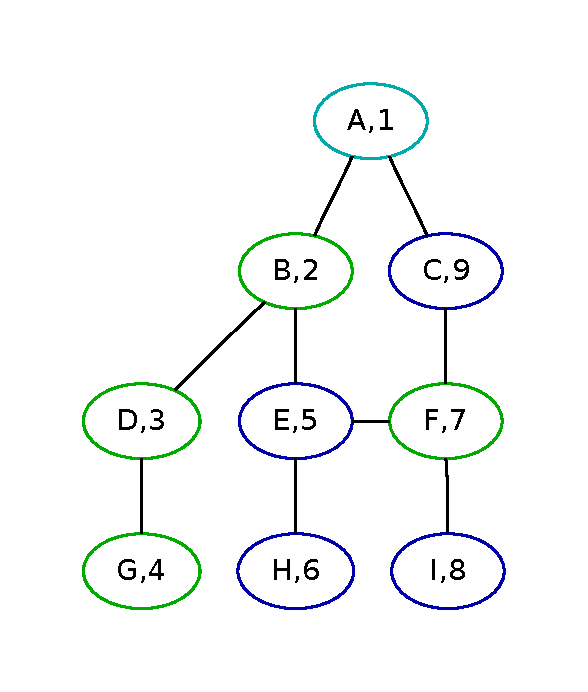
\includegraphics[width=.6\textwidth]{graphs/depth-first.pdf}
\caption{Dybde-først søgning i en graf}
\label{fig:depth-first}
\end{figure}


\subsubsection{Bredde-først søgning}
Ved bredde-først søgning (\textit{breadth-first search}) betragtes
første knude fra alle udgående kanter før deres kanter følges. Dermed
adskiller bredde-først søgning sig fra dybde-først søgning ved at søge
i niveauer af knuder (hvor dybde-først blot løb ned ad første knude).

Bredde-først søgning kan også beskrives på følgende måde:
\begin{enumerate}
\item Du står ved et vejkryds i en by og skal finde et specifikt
  vejkryds. Du har ikke noget kort.
\item På skift prøver du hver vej væk fra rundkørslen og ser om det
  efterfølgende vejkryds er det du søger. Du følger ikke de nye veje
  endnu.
\item Når du har noteret, at ingen af de umildbart næste vejkryds er
  det du søger, følger du deres respektive veje en ad gangen. Du
  noterer de kryds du møder, så du kan undgå at prøve dem igen senere.
\item Hvis krydset ikke var nede af den valgte retning afprøves næste vej.
\end{enumerate}

\Fref{fig:breadth-first} viser et eksempel på bredde-først
søgning. Grafen er den samme, som den i \fref{fig:depth-first}, men
knuderne er nu nummeret efter hvornår de opdages under en bredde-først
søgning.

\begin{figure}[h]\centering
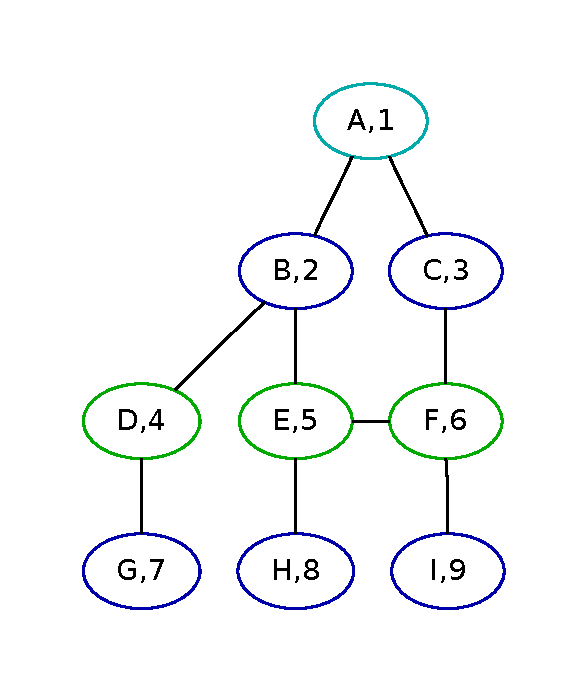
\includegraphics[width=.6\textwidth]{graphs/breadth-first.pdf}
\caption{Bredde-først søgning i en graf}
\label{fig:breadth-first}
\end{figure}


\section{Korteste vej}
\label{sec:shortest_path}

Korteste vej problemet (\textit{shortest path problem}) går ud på at
finde den korteste vej mellem to eller flere knuder i en
graf.

Problemet opstår i flere variationer:

\begin{enumerate}
\item \textbf{En til en:} Find den korteste vej mellem to knuder
\item \textbf{En til alle:} Find de korteste veje mellem \'en knude og
  alle andre knuder
\item \textbf{Alle til alle:} Find de korteste veje mellem alle par af
  knuder
\end{enumerate}

I de følgende afsnit skal vi se hvordan man kan løse den anden
variation. Nemlig hvordan man kan finde den korteste vej mellem en
udvalgt knude og alle andre knuder i grafen.

Når algoritmen er på plads skal vi se, hvordan den kan bruges til at
finde den korteste vej mellem to hustande i en by.


\subsection{Dijkstra's algoritme}

Dijkstra's algoritme løser \'en til alle korteste vej
problemet.

Første iteration af en bredde-først søgning afdækker alle knuder, der
har 1 kant til start-knuden. Anden iteration afdækker alle med 2
kanter. $n$'e iteration afdækker alle med $n$ kanter til
start-knuden. Vi kan nu tælle antaller af kanter til start-knuden ved
bredde-først søgning. \Fref{fig:dijkstra0} viser hvordan
kant-afstanden mellem knuden $A$ og alle andre knuder i grafen kan
findes ved brug af bredde-først søgning. Hvis alle kanter har vægten
$1$, er en til alle kortevej problemet nu løst.

\begin{figure}[h]\centering
\includegraphics[width=.49\textwidth]{graphs/dijkstra00.pdf}
\includegraphics[width=.49\textwidth]{graphs/dijkstra01.pdf}
\includegraphics[width=.49\textwidth]{graphs/dijkstra02.pdf}
\includegraphics[width=.49\textwidth]{graphs/dijkstra03.pdf}
\caption{Dybde-først søgning, der tæller kant-afstand til $A$}
\label{fig:dijkstra0}
\end{figure}

Vi udvider nu problemet med kanter. Da alle kanter var sat til $1$ var
det blot et spørgsmål om at lægge $1$ til hver gang vi begav os ud i
et nyt niveau. Det er ikke nok længere, da det ikke længere er
sikkert, at den korteste vej er den med det færreste antal kanter. I
stedet gør vi følgende observation:

Lad $K(XY)$ være længden af den korteste vej fra knude $X$ til knude
$Y$. For eksempel var $K(AC)=2$. Bemærk nu, at der om knude $C$
gælder, at
\[K(AC) = \min(K(AB)+1,K(AE)+1) \]

Den korteste vej fra $A$ til $C$ går altså enten gennem knude $B$
eller $E$ og må være $1$ højere end den laveste af deres afstande til
$A$.
Lad nu $K_i(AC)$ være den længden af den korteste vej fra $A$ til $C$
i iteration $i$. For eksempel er $K_0(AC)$ ukendt, mens $K_2(AC)=2$.

Lad nu $W(XY)$ være vægten mellem knuderne $X$ og $Y$. Da kan
ændringen i iteration $2$ beskrives ved:
\[ K_2(AC) = \min(K_1(AB) + W(BC), K_1(AC)) \]

Den korteste vej fra $A$ til $C$ i iteration $2$ er dermed enten den
korteste vej til $B$ plus vægten mellem $B$ og $C$ eller den korteste
vej til $C$ fra en anden knude.

Den korteste vej til en knude er altså minimum af de korteste veje til
de omkringliggende knuder + den pris det koster at følge den
mellemliggende kant.

\subsubsection{Gennemgang af algoritmen}
Dijkstra's algoritme virker på følgende måde:
\begin{enumerate}
\item Sæt afstanden til start-knuden til $0$ og afstanden til de andre
  knuder til $\infty$.
\item Tilføj start-knuden til en liste $L$ af knuder der skal besøges.
\item Udtag den knude $X$ fra listen $L$ der har den korteste afstand
  angivet (i første iteration vil det altid være start-knuden).
\item Opdater alle omkringliggende knuder, så deres afstand bliver den
  mindste af deres egen afstand og $X$'s afstand plus den
  mellemliggende kants vægt.

  Eller sagt på en anden måde:
  \[ K(AY) = \min(K(AY), K(AX)+W(XY)) \]
  hvor $Y$ er en omkringliggende knude og $XY$ er kanten mellem $X$ og
  $Y$.
\item Tilføj de omkringliggende knuder til $L$ hvis de ikke har været
  besøgt før.
\item Mark\'er $X$ som værende besøgt.
\item Gentag fra punkt 3 indtil listen $L$ er tom.
\end{enumerate}

\subsubsection{Eksempel}
\Fref{fig:dijkstraw0} viser et eksempel på Dijkstra's
algoritme. Farverne på figuren har følgende betydning:
\begin{itemize}
\item Sort: knuden er endnu ikke besøgt
\item Blå: knuden ligger i listen $L$ og venter på at blive besøgt
\item Grøn: knuden er blevet besøgt og dens angivne afstand er længden af
  den korteste vej
\end{itemize}

\begin{enumerate}
\item I første iteration opdateres alle knuder, der deler en kant med
  start-knuden $A$. $B$'s afstand bliver sat til $2$, $D$'s til $1$ og
  $E$'s til $4$. Det er ikke nødvendigvis deres korteste veje til $A$,
  men det er de korteste veje, hvis de kun må bruge \'en kant.

  $L$ (listen over knuder der skal besøges) indeholder knuderne
  $B,D,E$.

\item I anden iteration vælges $D$, fordi den har den laveste afstand
  til $A$ (nemlig 1). $D$ bliver dermed taget ud af listen $L$ og i
  stedet markeret som besøgt (grøn). Dens omkringliggende knuder
  opdateres. For eksempel sættes afstanden til $E$ nu til $2$ da $1+1
  < 4$ ($1$ fra $D$'s afstand og $1$ fra kantens vægt).

  Knuden $H$ har ikke været besøgt før og lægges derfor i listen
  $L$. $A$ bliver ikke tilføjet til listen (den har allerede været besøgt).

  $L$ indeholder nu knuderne $B,E,H$.

\item I tredje iteration vælges knuden $B$. Knuden $C$ tilføjes til
  listen $L$ og dennes afstand opdateres, da $2+1 < 7$. $L$ indeholder
  $C,E,H$.

\item I fjerde iteration er det $E$, der har den laveste afstand til
  $A$. Denne tages ud af listen og dens naboknuder opdateres. $H$ får
  afstanden $4$, da $2+2<5$. $B$ opdateres ikke, da $2+1\not< 2$. $L$
  indeholder $C,F,H$.
\end{enumerate}


\begin{figure}[h]\centering
\includegraphics[width=.49\textwidth]{graphs/dijkstra-weighted00.pdf}
\includegraphics[width=.49\textwidth]{graphs/dijkstra-weighted01.pdf}
\includegraphics[width=.49\textwidth]{graphs/dijkstra-weighted02.pdf}
\includegraphics[width=.49\textwidth]{graphs/dijkstra-weighted03.pdf}
\caption{Dijkstra's algoritme, første 4 iterationer}
\label{fig:dijkstraw0}
\end{figure}

\newpage

\begin{enumerate}
\item[5.] I den femte iteration vælges knuden $C$. Ingen knuder kan
  opdateres, da alle naboknuders afstande allerede er optimale
  (grønne).

\item[6.] I den sjette iteration vælges knuden $F$. Naboknuden $G$
  opdateres og får afstanden $9$. Listen $L$ indeholder nu $G,H$.


\item[7-8.] I de sidste to iterationer markeres $H$ og $G$ som
  besøgt. Ingen afstande opdateres. Algoritmen slutter, når alle
  knuder er besøgt.
\end{enumerate}

\begin{figure}[h]\centering
\includegraphics[width=.49\textwidth]{graphs/dijkstra-weighted04.pdf}
\includegraphics[width=.49\textwidth]{graphs/dijkstra-weighted05.pdf}
\includegraphics[width=.49\textwidth]{graphs/dijkstra-weighted06.pdf}
\includegraphics[width=.49\textwidth]{graphs/dijkstra-weighted07.pdf}
\caption{Dijkstra's algoritme, sidste 4 iterationer (fortsat)}
\label{fig:dijkstraw1}
\end{figure}



%\newpage
%\subsubsection{Korteste vej mellem to hustande}



%\section{Eksempler på grafer (Hvad kan det bruges til?!)}
%\subsection{Vennenetværk (ikke-orienteret graf)}
%\subsection{Telefonnumre (orienteret graf)}
%\subsection{Repræsentation af en sudoku som en graf}


\newpage
\section{Implementation af en graf i Python}
Nu hvor det ligger fast hvad en graf er og hvad den kan bruges det
ville det være rart med en implementation, som vi kan bruge i
Python-programmer.

I denne sektion vil vi igennem analyse (hvad skal det kunne?)
designovervejelser (hvordan skal den kunne det?) og implementation
(hvordan koder man det?) få opbygget et Python grafmodul.

\subsection{Analyse}
\label{sec:analyse}
I dette afsnit diskuteres funktionaliteten af en graf. Hvad skal den
kunne?

Kogt helt ned, skal et grafmodul besidde funktionalitet:
\begin{enumerate}
\item Oprettelse af en tom graf
\item Indsættelse af knuder i en graf
\item Sletning af knuder i en graf
\item Tilføjelse af kant mellem to knuder i en graf
\item Sletning af kant mellem to knuder i en graf
\end{enumerate}

Med disse funktioner kan vi opbygge og nedrive grafer. Men før de er
anvendelige er det nødvendigt også at kunne undersøge grafer. Følgende
funktionalitet omhandler netop dette:
\begin{enumerate}
\item Findes knude $k$ i grafen?
\item Er knude $k_1$ og knude $k_2$ forbundet af en kant?
\item Hvor mange knuder indeholder grafen?
\item Hvor mange kanter indeholder grafen?
\end{enumerate}


\subsection{Designovervejelser}
I analysen \fref{sec:analyse} gennemgik jeg funktionaliteten af en
graf. Nu vil jeg diskutere hvordan denne funktionalitet kan
implementeres i Python.

Eftersom mine funktionaliteter beskæftiger sig med en specifik instans
af en graf, vælger jeg at lave en klasse \ct{Graf}, der
repræsentere en graf med de beskrevne muligheder. Hver funktionalitet
implementeres som en metode, der arbejder på grafen.

Inden jeg kan gå i gang med at beskrive, hvordan en graf kan ændres,
skal jeg først vælge en repræsentation af en graf. Hvordan kan skal
grafobjektet holde styr på knuder og kanter?

Der er følgende traditionelle måder at gøre dette på:
\begin{enumerate}
\item Hver knude indeholder en liste af andre knuder, som den er
  forbundet til.
\item Hver kant består af et par knuder, som denne forbinder.
\item En matrix af $($knuder $\times$ knuder$)$ angiver om et given
  par er forbundet\footnote{tænk på matricen som en liste af
    lister, der hver har et element for hver knude.}.
\end{enumerate}

Den første løsning kan implementeres med en \ct{Knude}-klasse, som
beskriver en knude. Det eneste knuden skal indeholde er sin egen
værdi, samt en liste over andre knuder, som den er forbundet til. At
undersøge om to knuder er forbundet kan gøres ved at løbe deres lister
igennem og se om de har hinanden som element. Køretiden for
operationen afhænger af hvor mange elementer de to knuder er forbundet
til.

Den anden løsning kan implementeres med en \ct{Kant}-klasse der
indeholder et par af knuder (de to kunder, som kanten
forbinder). \ct{Graf}-klassen skal nu indeholde en liste af knuder
sammen med en liste af kanter. At undersøge om to knuder er forbundet
af en kant kan gøres ved at løbe listen af kanter igennem og for hver
kant undersøge om de to knuder passer med parret. Køretiden er
afhænger nu af det samlede antal kanter i grafen.

Den tredje løsning kan også implementeres med lister, selvom den er
tænkt til matricer. Her behøves hverken en \ct{Kant}- eller
\ct{Knude}-klasse. \ct{Graf}-klassen indeholder en liste af knuder,
der hver har en liste af knuder. Hvis der findes en kant fra knude
nummer $1$ til knude nummer $2$ vil det andet element i den første
liste være \ct{sand} (f.eks.: \ct{kanter[1][2] == True}). Hvis kanten
ikke findes vil værdien være \ct{falsk} (altså: \ct{kanter[1][2] ==
  False}). Køretiden afhænger (grundet valget af lister) af antaller
af knuder og bliver dermed $O(k)$.\ \footnote{med matricer kan
  køretiden reduceres til $O(1)$.}\\

Jeg vælger at implementere model nummer et på grund af dens
simplicitet. I det følgende beskriver jeg hvordan jeg implementere
hver enkelte funktionalitet.

\subsubsection{Implementation af metoder}
\paragraph{Opret tom graf}
Den tomme graf er et \ct{Graph}-objekt uden nogen tilhørende
knuder. Listen af knuder er sat til den tomme liste. En tom graf kan
oprettes ved at instansiere klassen \ct{Graph}. Dennes \ct{\_\_init\_\_}
metode sætter listen af knuder til den tomme liste:
{\small
\begin{verbatim}
class Graph:
  ...
  def __init__(self):
    self.nodes = []
\end{verbatim}}

\paragraph{Indsættelse af knude}
En knude kan indsættes med \ct{Graph}-metoden
\ct{add\_node(node)}. Metoden virker ved at tilføje den nye knude til
grafens liste over knuder:
{\small
\begin{verbatim}
class Graph:
  ...
  def add_node(self, node):
    self.nodes.append(node)
\end{verbatim}}

\paragraph{Sletning af knude}
En knude kan fjernes fra en graf med \ct{Graph}-metoden
\ct{del\_node}. Metoden virker ved at fjerne knuden fra grafens list af
knuder:
{\small
\begin{verbatim}
class Graph:
  ...
  def del_node(self, node):
    self.nodes.remove(node)
\end{verbatim}}

\paragraph{Tilføjelse af kant}
En kant fra knude $a$ til knude $b$ kan tilføjes, ved at tilføje knude
$b$ til listen over kanter i knude $a$.

{\small
\begin{verbatim}
class Graph:
  ...
  def add_edge(self, node_a, node_b):
    node_a.add_edge(node_b)
\end{verbatim}}

I \ct{Node}-klassen tilføjer \ct{add\_edge} metoden knuden til dens
liste over kanter:
{\small
\begin{verbatim}
class Node:
  ...
  def add_edge(self, node):
    self.edges.append(node)
\end{verbatim}}

\paragraph{Sletning af kant}
En kan fra knude $a$ til knude $b$ kan slettes, ved at fjerne knude
$b$ fra listen over kanter i knude $a$.

{\small
\begin{verbatim}
class Graph:
  ...
  def del_edge(self, node_a, node_b):
    node_a.del_edge(node_b)
\end{verbatim}}

I \ct{Node}-klassen fjernes knuden fra listen over kanter:
{\small
\begin{verbatim}
class Node:
  ...
  def del_edge(node):
    self.edges.remove(node)
\end{verbatim}}


\paragraph{Findes knude $k$ i grafen?}
Hvis knude $k$ ligger i grafen, ligger den i listen over knuder:

{\small
\begin{verbatim}
class Graph:
  ...
  def has_node(self, node):
    return (node in self.nodes)
\end{verbatim}}

\paragraph{Findes en kant fra knude $k_1$ til knude $k_2$?}
Hvis en kan findes fra knude $k_1$ til knude $k_2$ må knude $k_2$
ligge i listen over $k_1$'s kanter:
{\small
\begin{verbatim}
class Graph:
  ...
  def has_edge(node_a, node_b):
    return node_a.has_edge(node_b)
\end{verbatim}}

I \ct{Node}-klassen testes om \ct{node\_b} ligger i listen over kanter:
{\small
\begin{verbatim}
class Node:
  ...
  def has_edge(self, node):
    return (node in self.edges)
\end{verbatim}}

\paragraph{Hvor mange knuder indeholder grafen?}
Antallet af knuder i grafen er det samme som længden af listen over
knuder:
{\small
\begin{verbatim}
class Graph:
  ...
  def count_nodes(self):
    return len(self.nodes)
\end{verbatim}}

\paragraph{Hvor mange kanter indeholder grafen?}
Antallet af kanter i grafen er lig med antallet af fra de enkelte
knuder:
{\small
\begin{verbatim}
class Graph:
  ...
  def count_edges(self):
    count = 0
    for node in self.nodes:
      count += node.count_edges()
    return count
\end{verbatim}}

I \ct{Node}-klassen tælles antallet af kanter ved at tælle antallet af
elementer i listen over kanter:
{\small
\begin{verbatim}
class Node:
  ...
  def count_edges(self):
    return len(self.edges)
\end{verbatim}}


\subsubsection{Fejlhåndtering}
Flere af ovenstående punkter kan give en fejl. Man kan forsøge at
fjerne en knude der ikke findes, eller tilføje en kant der findes i
forvejen. I dette afsnit vil jeg belyse de metoder der kan fejle, og
udvide dem med fejlhåndtering.

\paragraph{Definition af fejl:}
Til at starte med definerer jeg fire fejltyper (\ct{exceptions}), som
grafen kan \textit{kaste} i tilfælde af fejl:
{\small
\begin{verbatim}
class NodeAlreadyExistsError(Exception):
    """ Knuden findes allerede """
    pass

class NoSuchNodeError(Exception):
    """ Knuden findes ikke """
    pass

class EdgeAlreadyExistsException(Exception):
    """ Kanten findes allerede """
    pass

class NoSuchEdgeError(Exception):
    """ Kanten findes ikke """
    pass
\end{verbatim}}

\paragraph{Implementation af fejlhåndtering:}
Jeg ændrer de problematiske metoder, så de nu kaster en af
ovenstående fejl, når en ulovlig handling forsøges.\\

Argumentet til \ct{add\_node} skal være en knude, som ikke ligger i
grafen:
{\small
\begin{verbatim}
def add_node(node):
  # Fejlhåndtering
  if node in self.nodes:
    raise NodeAlreadyExistsError(node)
  # Tilføj knuden
  self.nodes.append(node)
\end{verbatim}}

Argumentet til \ct{del\_node} skal være en knude, som findes i grafen:
{\small
\begin{verbatim}
def def_node(node):
  # Fejlhåndtering
  if not node in self.nodes:
    raise NoSuchNodeError(node)
  # Slet knude
  self.nodes.remove(node)
\end{verbatim}}

\paragraph{Smartere fejlhåndtering:}
Jeg ser, at fejlhåndteringen tager følgende form:
\begin{enumerate}
\item Undersøg om en knude eller kant findes eller ej
\item Kast fejl hvis det ikke passer med forventningen
\end{enumerate}

Ved at definere en generel metode for dette, kan jeg reducere antallet
af linjer brugt på fejlhåndtering betydeligt. Jeg definerer en
funktion for knude og en for kanter. Jeg vælger at kalde dem
\ct{ensure\_nodes} og \ct{ensure\_edges}:

\begin{samepage}
{\small
\begin{verbatim}
class Graph:
  ...

  def ensure_nodes(self, nodes, must_exist):
      """ Kast en fejl hvis en af knuderne findes/ikke findes """
      for node in nodes:
          exists = self.has_node(node)
          if must_exist and not exists:
              raise NoSuchNodeError(node)
          if not must_exist and exists:
              raise NodeAlreadyExistsError(node)

  def ensure_edges(self, edges, must_exist):
      """ Kast en fejl hvis en af kanterne findes/ikke findes """
      for node_a, node_b in edges:
          exists = self.has_edge(node_a, node_b)
          if must_exist and not exists:
              raise NoSuchEdgeError((node_a, node_b))
          if not must_exist and exists:
              raise EdgeAlreadyExistsError((node_a, node_b))
\end{verbatim}}
\end{samepage}


Jeg kan nu skrive fejlhåndteringen for \ct{add\_node} og \ct{del\_node}
således:

{\small
\begin{verbatim}
def add_node(node):
  # Fejlhåndtering
  self.ensure_nodes( [node], True )
  # Tilføj knuden
  self.nodes.append(node)

def def_node(node):
  # Fejlhåndtering
  self.ensure_nodes( [node], False )
  # Slet knude
  self.nodes.remove(node)
\end{verbatim}}

Bemærk, at der kun bruges en enkelt linje til fejlhåndtering i den nye
kode. Jeg fortsætter med at tilføje fejlhåndtering til de andre
kritiske metoder: \\

Argumenterne til \ct{add\_edge} skal være to knuder, der findes i
grafen (der må gerne findes en kant i forvejen):
{\small
\begin{verbatim}
class Graph:
  ...
  def add_edge(self, node_a, node_b):
    # Fejlhåndtering
    self.ensure_nodes(  [node_a, node_b]  , True  )
    # Tilføj kant
    node_a.add_edge(node_b)
\end{verbatim}}

Argumenterne til \ct{del\_edge} skal være to knuder, der deler en
kant:
{\small
\begin{verbatim}
class Graph:
  ...
  def del_edge(self, node_a, node_b):
    # Fejlhåndtering
    self.ensure_edges( [(node_a, node_b)], True )
    # Slet kant
    node_a.del_edge(node_b)
\end{verbatim}}


\subsection{Test og afprøvning}


\subsection{Endelig Implementation (kildekode)}
\begin{alltt}
\input{code/graph.py}
\end{alltt}

\end{document}

